\chapter{Self-Supervised Learning}

\section{Motivation}

For many years, supervised learning dominated artificial intelligence because it achieved remarkable performance on tasks such as image classification, speech recognition, and machine translation. However, as deep learning models became larger, their demand for labeled data increased dramatically. Although billions of images and trillions of words are freely available on the Internet, only a small fraction of this data is manually labeled. Creating high-quality labels requires significant time, financial resources, and often the expertise of domain specialists, making supervised learning difficult to scale. This limitation motivated researchers to search for a new learning paradigm capable of exploiting the enormous amount of unlabeled data available while reducing the dependence on manual annotation.


\section{Why Not Simply Use Unsupervised Learning?}

Unsupervised learning had existed long before self-supervised learning, but its objective is fundamentally different. Traditional unsupervised methods focus on discovering hidden structures in data through clustering, dimensionality reduction, or density estimation. Although these techniques reveal patterns, they do not necessarily produce representations that are useful for tasks such as classification or detection. Researchers therefore sought a method that could learn discriminative representations while still avoiding manual labels.

Self-Supervised Learning (SSL) is a learning paradigm in which the supervision signal is generated automatically from the data itself, instead of relying on human annotations. The model creates its own prediction task, known as a pretext task, and learns meaningful representations by solving it. In this way, SSL combines the scalability of unsupervised learning with the representation quality of supervised learning.

\section{What Does SSL Actually Learn?}

Unlike supervised learning, whose immediate goal is to predict labels, SSL aims to learn representations. A representation is a feature vector (embedding) that captures the semantic information contained in the input. Once these representations are learned, they can be transferred to many downstream tasks such as classification, object detection, segmentation, retrieval, and medical image analysis.

Since unlabeled data is vastly more abundant than labeled data, self-supervised learning has become the preferred strategy for training modern foundation models. Today, many of the most influential AI systems---including \textbf{BERT}, \textbf{DINOv2}, \textbf{MAE}, and even \textbf{GPT} through next-token prediction---rely on self-supervised learning during pretraining.

\section{Pretext Tasks}

A pretext task is an artificial task created from the data itself.

\begin{table}[H]
\centering
\caption{Examples of Methods and Their Pretext Tasks}
\label{tab:pretext_tasks}
\begin{tabularx}{\textwidth}{lX}
\toprule
\textbf{Method} & \textbf{Pretext Task} \\
\midrule
\textbf{BERT} & Predict masked words \\
\textbf{MAE} & Reconstruct masked image patches \\
\textbf{SimCLR} & Match two augmented views \\
\textbf{DINO} & Match teacher-student representations \\
\bottomrule
\end{tabularx}
\end{table}

The model learns meaningful features while solving the pretext task. After SSL pretraining, the learned encoder is reused for real applications called downstream tasks, e.g., classification, object detection, face recognition. The SSL encoder is usually fine-tuned with a much smaller labeled dataset.

\section{The Two Main Families of SSL}

\begin{enumerate}[label=\Roman*)]
    \item \textbf{Contrastive Learning}: Learn by comparing representations.
    \begin{itemize}
        \item \textbf{SimCLR}
        \item \textbf{MoCo}
        \item \textbf{BYOL}
        \item \textbf{DINO}
    \end{itemize}
    
    \item \textbf{Masked / Reconstruction Learning}: Learn by reconstructing missing information.
    \begin{itemize}
        \item \textbf{BEiT}
        \item \textbf{MAE}
        \item \textbf{iBOT} (hybrid approach)
    \end{itemize}
\end{enumerate}

These two families dominate modern self-supervised vision research.

\section{Contrastive Learning}

The goal of S.S.L is to learn meaningful representations without labels. The question then becomes: can we tell the model which images are similar and which are different?

Contrastive learning solves this problem by creating its own supervision. Instead of learning from class labels, it learns by comparing different views of the data. The model is trained to bring representations of similar samples closer together while pushing representations of different samples farther apart in the embedding space.

\subsection{Positive Pairs}

A positive pair consists of two different views of the same sample. For example, given an image $x$, we apply two random augmentations:
\begin{itemize}
    \item Random Crop
    \item Color Jitter
    \item Gaussian Blur
    \item Horizontal Flip
\end{itemize}

Producing:
\begin{figure}[H]
\centering
\begin{tikzpicture}[
node distance=1.8cm,
>=Stealth,
every node/.style={font=\small},
box/.style={draw, rounded corners, minimum width=2.4cm, minimum height=0.8cm, align=center},
pair/.style={draw, fill=blue!10, rounded corners, minimum width=2.8cm, minimum height=0.9cm}
]

% Top branch
\node[box] (img1) {Image 1};
\node[box, right=of img1] (crop) {Cropping};
\node[box, right=of crop] (emb1) {Embedding};

% Bottom branch
\node[box, below=1.5cm of img1] (img2) {Image 1};
\node[box, right=of img2] (flip) {Flip};
\node[box, right=of flip] (emb2) {Embedding};

% Pair
\node[pair, right=2.5cm of emb1, yshift=-0.75cm] (pair) {Positive Pair};

% Arrows
\draw[->] (img1) -- (crop);
\draw[->] (crop) -- (emb1);
\draw[->] (img2) -- (flip);
\draw[->] (flip) -- (emb2);

\draw[->] (emb1) -- (pair);
\draw[->] (emb2) -- (pair);

\end{tikzpicture}
\caption{Construction of a positive pair.}
\end{figure}

Although the two images look different, they originate from the same image and therefore form a positive pair. The model should produce similar embeddings for both views.

\subsection{Negative Pairs}

A negative pair consists of two views coming from different samples.
\begin{figure}[H]
\centering
\begin{tikzpicture}[
node distance=2cm,
>=Stealth,
every node/.style={font=\small},
box/.style={draw, rounded corners, minimum width=2.4cm, minimum height=0.8cm, align=center},
pair/.style={draw, fill=red!10, rounded corners, minimum width=2.8cm, minimum height=0.9cm}
]

\node[box] (cat) {Cat Image};
\node[box, right=of cat] (emb1) {Embedding};

\node[box, below=1.5cm of cat] (dog) {Dog Image};
\node[box, right=of dog] (emb2) {Embedding};

\node[pair, right=2.5cm of emb1, yshift=-0.75cm] (pair) {Negative Pair};

\draw[->] (cat) -- (emb1);
\draw[->] (dog) -- (emb2);

\draw[->] (emb1) -- (pair);
\draw[->] (emb2) -- (pair);

\end{tikzpicture}
\caption{Construction of a negative pair.}
\end{figure}

Since the two images represent different objects, their embeddings should be separated in the embedding space.

The objective is therefore:
\begin{itemize}
    \item Positive pairs $\longrightarrow$ close together.
    \item Negative pairs $\longrightarrow$ far apart.
\end{itemize}

\begin{figure}[H]
    \centering
    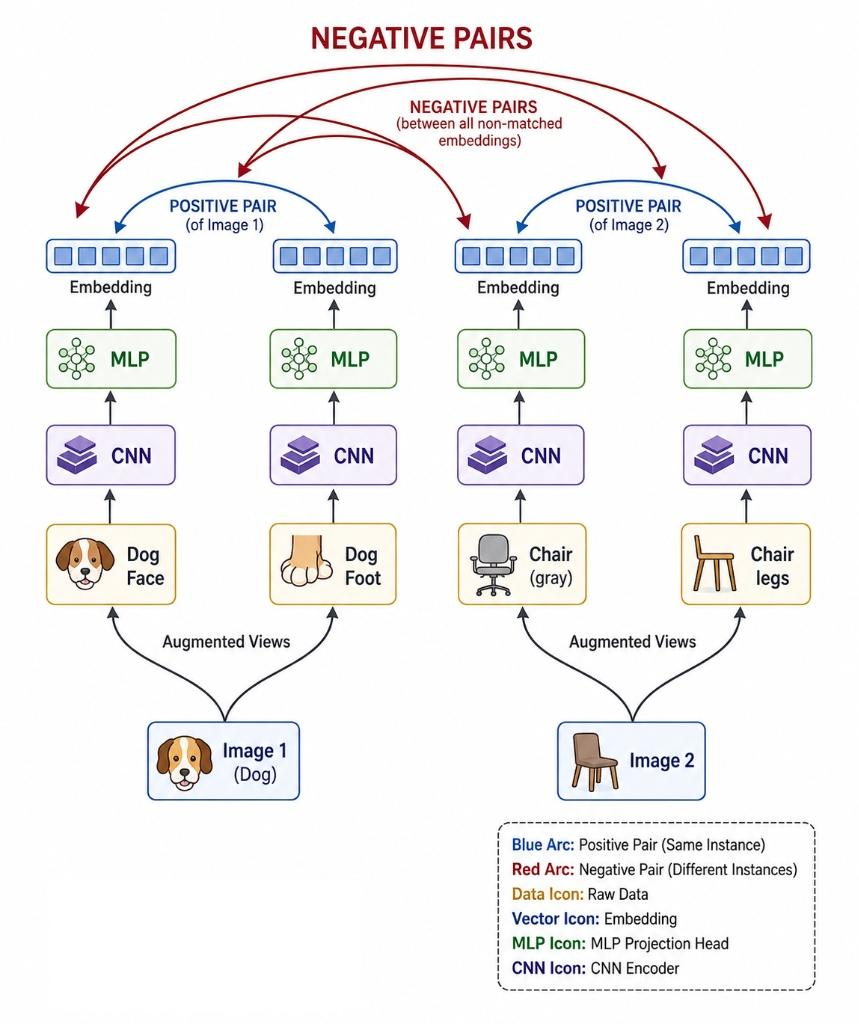
\includegraphics[width=0.92\textwidth]{figures/fig_7_contrastive_pairs.jpg}
    \caption{Contrastive Learning Framework with Positive and Negative Pairs.}
    \label{fig:contrastive_pairs}
\end{figure}

\section{Data Augmentation as Supervision}

In supervised learning, labels provide the supervision. In contrastive learning, data augmentation becomes the supervision.

By generating multiple views of the same image, the model automatically knows which samples should be considered similar, eliminating the need for manual annotations.

Common augmentations include:
\begin{itemize}
    \item Random Crop
    \item Random Resize
    \item Horizontal Flip
    \item Color Jitter
    \item Gaussian Blur
    \item Random Grayscale
\end{itemize}

The quality of these augmentations is one of the most important factors affecting S.S.L performance.

The model does not compare images directly; instead, it compares their embeddings.

The goal is to organize this space so that:
\begin{itemize}
    \item Similar images have nearby embeddings.
    \item Different images have distant embeddings.
\end{itemize}

To measure the similarity between two embeddings, contrastive learning typically uses cosine similarity:
\[
\text{Sim}(z_i, z_j) = \frac{z_i \cdot z_j}{\|z_i\| \cdot \|z_j\|}
\]
Most SSL methods normalize embeddings before computing cosine similarity.

\section{InfoNCE Loss}

The InfoNCE (Information Noise Contrastive Estimation) Loss is the objective function used in most contrastive learning methods. Its purpose is to learn an embedding space where positive pairs are close together and negative pairs are far apart.

For an anchor embedding $z_i$, a positive embedding $z_j$, and a set of negative embeddings, the InfoNCE Loss is:
\[
L_i = -\log \left( \frac{\exp\left( \frac{\text{sim}(z_i, z_j)}{\tau} \right)}{\sum_{k=1}^{K} \exp\left( \frac{\text{sim}(z_i, z_k)}{\tau} \right)} \right)
\]
where:
\begin{itemize}
    \item $z_i$: anchor embedding
    \item $z_j$: positive embedding
    \item $z_k$: all candidate embeddings (Positive + Negative)
    \item $\text{sim}$: cosine similarity
    \item $\tau$: temperature parameter
\end{itemize}

The numerator $\exp\left( \frac{\text{sim}(z_i, z_j)}{\tau} \right)$ contains the similarity between the anchor and its positive pair, which the model wants to maximize.

The denominator $\sum_{k} \exp\left( \frac{\text{sim}(z_i, z_k)}{\tau} \right)$ contains the similarity between the anchor and all candidate samples, including the positive and all negatives.

Minimizing the InfoNCE Loss therefore encourages the model to:
\begin{itemize}
    \item Increase the similarity between positive pairs.
    \item Decrease the similarity between negative pairs.
\end{itemize}

As training progresses, the embedding space becomes organized so that semantically similar samples are clustered together while dissimilar samples are separated.

\subsection{Temperature Parameter \texorpdfstring{($\tau$)}{(tau)}}

Before applying the Softmax in InfoNCE, similarities are divided by a temperature parameter ($\tau$): $\frac{\text{sim}(z_i, z_j)}{\tau}$. The temperature controls how strongly the model distinguishes between similar and dissimilar samples.
\begin{itemize}
    \item Small $\tau$: sharper probability distribution, stronger separation.
    \item Larger $\tau$: smoother distribution, weaker separation.
\end{itemize}

It is simply a hyperparameter used during training.

\subsection*{Summary}
Contrastive Learning enables self-supervised learning by comparing representations, instead of relying on labels. It creates positive pairs from different augmentations of the same sample and negative pairs from different samples. Images are mapped into an embedding space, where cosine similarity measures how close two embeddings are. The InfoNCE loss encourages positive pairs to become similar and negative pairs to become dissimilar, while the temperature parameter controls the sharpness of this optimization. These principles form the foundation of methods such as: \textbf{SimCLR}, \textbf{MoCo}, \textbf{BYOL}, and \textbf{DINO}.

\section{SimCLR (Simple Framework for Contrastive Learning of Visual Representations)}

Before \textbf{SimCLR}, contrastive learning methods often relied on complex architectures, memory banks, or specialized training procedures. In 2020, Google Research introduced \textbf{SimCLR}, demonstrating that a simple framework based on strong data augmentation, a projection head, and a contrastive loss could learn powerful visual representations without labels. \textbf{SimCLR} became the foundation for many later SSL methods.

The core idea of \textbf{SimCLR} is straightforward: generate two different augmented views of the same image, encode them into embeddings, and train the model to make these embeddings similar while separating them from embeddings of other images.

Thus, supervision comes entirely from the augmentations.

\begin{figure}[H]
    \centering
    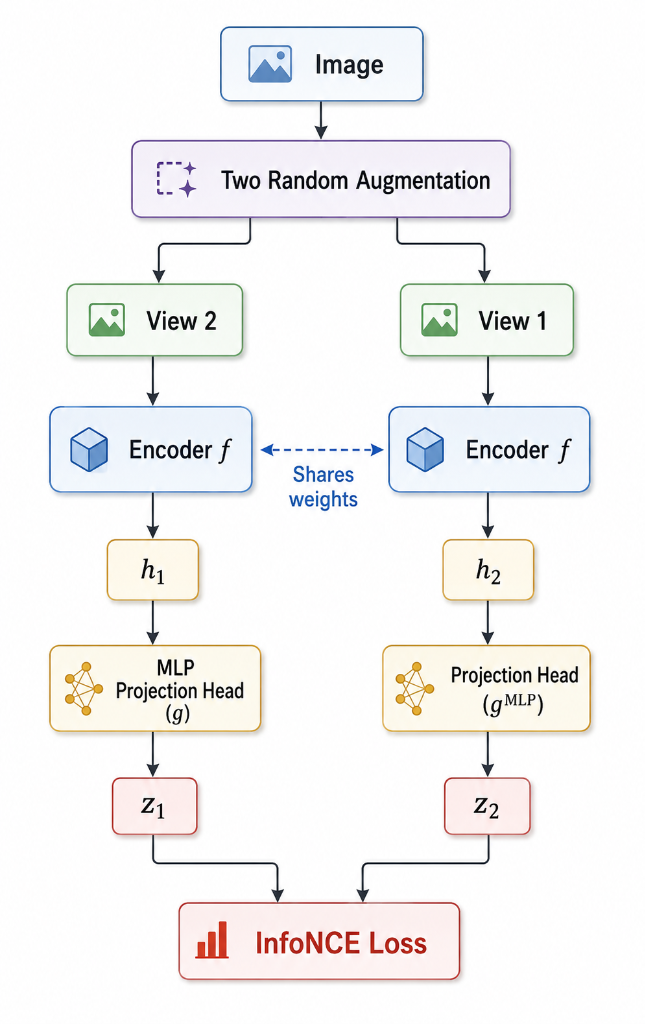
\includegraphics[width=0.75\textwidth]{figures/fig_7_simclr_architecture.png}
    \caption{SimCLR Architecture Overview.}
    \label{fig:simclr_architecture}
\end{figure}

The two encoder branches share the same parameters.

Each input image is transformed twice using random augmentations. Typical augmentations include: Random Crop, Random Resize, Horizontal Flip, Color Jitter, Gaussian Blur, Random Grayscale. The two resulting images form a positive pair.

The encoder extracts visual features from each augmented image. Originally, \textbf{SimCLR} used a standard CNN such as ResNet-50, although any backbone can be used. The encoder produces a feature representation $h = f(x)$ where:
\begin{itemize}
    \item $x = \text{augmented img}$
    \item $h = \text{learned feature representation}$
\end{itemize}

One of \textbf{SimCLR}'s most important contributions is the Projection Head. Instead of computing the contrastive loss directly on the encoder output, \textbf{SimCLR} introduces a small MLP $z = g(h)$. Researchers found that applying the contrastive loss directly on the encoder representation reduces downstream performance.

(The encoder learns useful visual representations by maximizing agreement between different augmented views of the same image).

The projection head separates:
\begin{itemize}
    \item Representation learning (encoder output $h$)
    \item Contrastive optimization (projected embedding $z$)
\end{itemize}

After training:
\begin{itemize}
    \item The projection head is discarded.
    \item Only the encoder is kept.
\end{itemize}

This improves transfer learning performance.

The projected embeddings $z_1, z_2$ are normalized and compared using cosine similarity. The InfoNCE loss then:
\[
L = -\log \left( \frac{\exp\left( \frac{\text{sim}(z_1, z_2)}{\tau} \right)}{\sum_k \exp\left( \frac{\text{sim}(z_1, z_k)}{\tau} \right)} \right)
\]
\begin{itemize}
    \item Maximizes similarity between positive pairs.
    \item Minimizes similarity with all negative pairs in the batch.
\end{itemize}

\subsection{Batch Training}

\textbf{SimCLR} does not use a memory bank (images stocked in memory that always play the role of negative pairs).

Instead, all other images in the mini-batch serve as negative samples.

For a batch of $N$ images:
\begin{itemize}
    \item Two augmentations are created.
    \item Total samples become $2N$.
    \item Each sample has one positive pair.
    \item The remaining $2N - 2$ samples are negatives.
\end{itemize}

As a result, larger batch sizes provide more negative samples and generally improve representation learning.

\subsection{Advantages}

\textbf{SimCLR} demonstrated that strong self-supervised representations can be learned using a simple framework.

Advantages include:
\begin{itemize}
    \item No labeled data required.
    \item Simple architecture.
    \item Strong downstream performance.
    \item Easy to implement.
    \item Foundation for many later S.S.L methods.
\end{itemize}

\subsection{Limitations}

\begin{itemize}
    \item Requires very large batch size.
    \item Large GPU memory consumption.
    \item Performance depends heavily on data augmentation.
    \item No memory bank for storing negatives.
\end{itemize}

These limitations motivated the development of \textbf{MoCo}.

\section{MoCo (Momentum Contrast)}

Although \textbf{SimCLR} demonstrated that contrastive learning could learn powerful visual representations, it had a major limitation: it required extremely large batch sizes. To provide enough negative samples, training \textbf{SimCLR} often required multiple GPUs and thousands of images per batch, making it impractical for many researchers.

To overcome this limitation, Facebook AI introduced Momentum Contrast (\textbf{MoCo}) in 2020. Instead of relying on large batches, \textbf{MoCo} maintains a dynamic dictionary of negative samples using a memory queue and a momentum encoder.

The key idea behind \textbf{MoCo} is simple: instead of generating negative samples only from the current mini-batch, maintain a large queue of embeddings computed from previous mini-batches. This allows the model to use thousands of negative samples while training with relatively small batch sizes.

\begin{figure}[H]
    \centering
    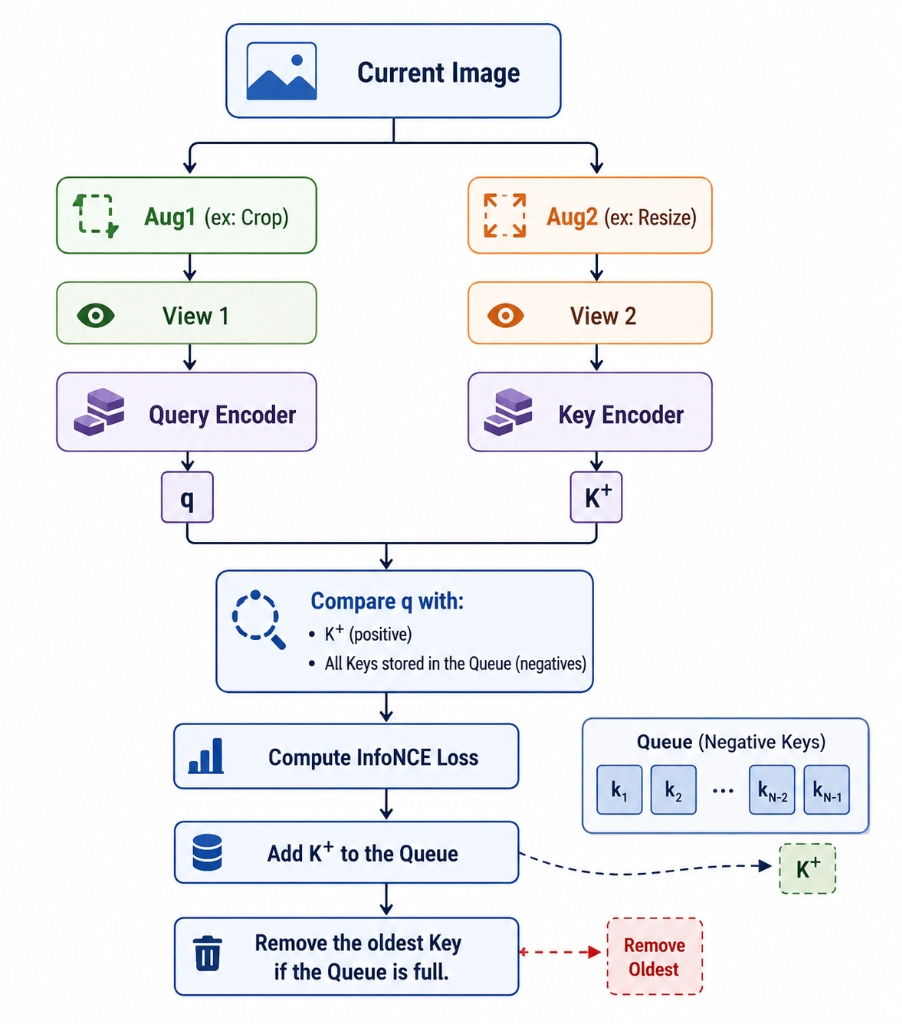
\includegraphics[width=0.82\textwidth]{figures/fig_7_moco_architecture.jpg}
    \caption{MoCo (Momentum Contrast) Architecture Overview.}
    \label{fig:moco_architecture}
\end{figure}

Unlike \textbf{SimCLR}, the two encoders do not share weights directly.

\subsection{MoCo Training Process}

\subsubsection{Step 1: Generate Two Views}
A training image is randomly augmented twice, producing two different views of the same image. These two views form a positive pair.
\[
\text{img} \longrightarrow \text{View 1}, \quad \text{View 2}
\]

\subsubsection{Step 2: Compute the Query Embedding}
The first view is passed through the Query Encoder, which is the main network being trained.

The query embedding is computed as:
\[
q = f_q(x)
\]
The Query Encoder parameters are updated normally using backpropagation after each training iteration.

\subsubsection{Step 3: Compute the Positive Key}
The second view is passed through the Momentum Encoder, which is not updated by gradient descent. Instead, its parameters are updated using an Exponential Moving Average (EMA) of the Query Encoder:
\[
\theta_K = m \theta_K + (1 - m) \theta_q
\]
where:
\begin{itemize}
    \item $\theta_q$ are the Query Encoder parameters.
    \item $\theta_K$ are the Momentum Encoder parameters.
    \item $m$ is the momentum coefficient (typically 0.999).
\end{itemize}

This slow update keeps the key representations stable during training.
\[
\text{View 2} \longrightarrow \text{Momentum Encoder} \longrightarrow \text{Positive Key } (K^+)
\]

\subsubsection{Step 4: Retrieve Negative Samples}
\textbf{MoCo} introduces a Memory Queue, which stores key embeddings generated during previous training iterations.
\[
\text{Memory Key}: [K_1], [K_2], [K_3], \dots, [K_n]
\]
Instead of using only the current mini-batch as in \textbf{SimCLR}, \textbf{MoCo} retrieves all the embeddings stored in this queue. These embeddings serve as the negative samples.

\subsubsection{Step 5: Compute the Contrastive Loss}
For each query embedding, the model compares:
\begin{itemize}
    \item The corresponding positive key $K^+$.
    \item All negative keys stored in the memory queue.
\end{itemize}

\[
\begin{array}{c|l c}
q & K^+ & (\text{Positive}) \quad \checkmark \\
  & K_1 & (\text{Negative}) \quad \times \\
  & K_2 & (\text{Negative}) \quad \times \\
  & K_3 & (\text{Negative}) \quad \times \\
  & \dots &
\end{array}
\]

The InfoNCE Loss encourages the query to become closer to its positive key while moving away from all negative keys.

\subsubsection{Step 6: Update the Models}
After computing the InfoNCE loss:
\begin{itemize}
    \item The Query Encoder is updated through backpropagation.
    \item The Momentum Encoder is updated using the EMA equation rather than gradients.
\end{itemize}

This ensures that the key embeddings evolve smoothly over time.

\subsubsection{Step 7: Update the Memory Queue}
Finally, the newly computed positive $K^+$ is inserted into the memory queue. If the queue is full, the oldest embedding is removed.
\[
\text{Queue Before}: [K_1], [K_2], [K_3], \dots, [K_n] \rightsquigarrow \text{Queue After}: [K_2], [K_3], [K_4], \dots, [K_n], [K^+]
\]

The queue therefore acts as a dynamic dictionary of negative samples, allowing \textbf{MoCo} to train with small mini-batches while benefiting from a large number of negatives.

\subsection{Why Use a Momentum Encoder?}

If the queue were generated by a rapidly changing encoder, key representations in the queue would become inconsistent across training iterations, causing loss computation instability. The Momentum Encoder evolves slowly through EMA updates, ensuring that embeddings in the queue remain relatively stable and improving the quality of the contrastive learning process.

\subsection{Advantages}

Compared with \textbf{SimCLR}:
\begin{itemize}
    \item Small mini-batches are sufficient.
    \item Large number of negative samples.
    \item Lower GPU memory requirements.
    \item More efficient training.
    \item High-quality representations.
\end{itemize}

\subsection{Limitations}

Despite its success, \textbf{MoCo} still relies on negative samples:
\begin{itemize}
    \item Selecting effective negatives.
    \item False negatives (different images representing similar semantics).
    \item Dependence on contrastive loss.
\end{itemize}

These limitations motivated researchers to explore negative-free learning, leading to methods such as \textbf{BYOL}.

\section{Why Contrastive Learning Isn't Enough?}

Contrastive Learning successfully learns visual representations by comparing positive and negative pairs, but it suffers from several limitations. It often requires large numbers of negative samples, leading to high computational costs. Additionally, some negatives are difficult to distinguish (hard negatives), while others are incorrectly treated as negatives despite sharing similar semantics (false negatives). Although negative samples prevent representation collapse, they also introduce complexity into the training process. These challenges motivated researchers to explore whether effective self-supervised learning could be achieved without any negative samples, leading to the development of \textbf{BYOL}.

\section{BYOL (Bootstrap Your Own Latent)}

Contrastive learning methods such as \textbf{SimCLR} and \textbf{MoCo} learn representations by comparing positive and negative pairs. Although effective, they require carefully selecting negative samples and suffer from problems such as false negatives and high computational cost.

In 2020, DeepMind introduced \textbf{BYOL}, showing that high-quality representations can be learned without using any negative samples. This result was surprising because it challenged the common belief that negative pairs were essential to prevent representation collapse.

\subsection{The Key Idea of BYOL}

Instead of pushing different images apart, \textbf{BYOL} learns by making two networks produce similar representations of two augmented views of the same image.

Unlike \textbf{SimCLR} or \textbf{MoCo}:
\begin{itemize}
    \item No Negative pairs
    \item No Memory Queue
    \item No Contrastive Loss
\end{itemize}

The model simply learns to predict its own representation.

\begin{figure}[H]
    \centering
    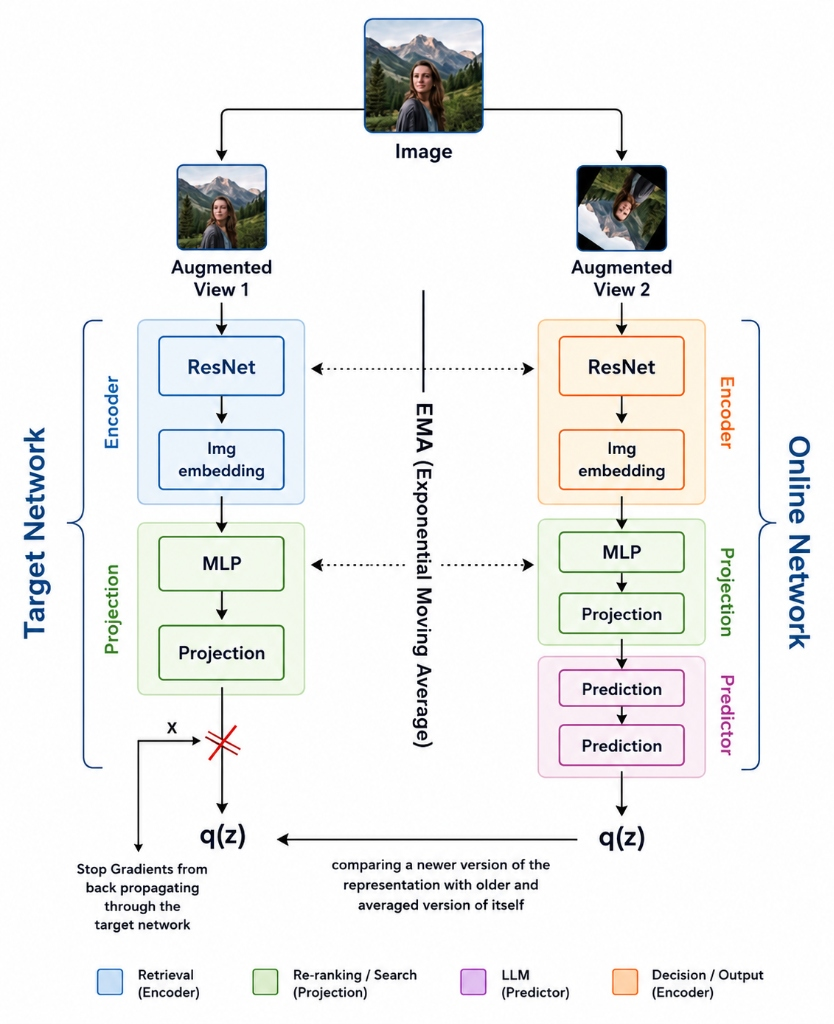
\includegraphics[width=0.82\textwidth]{figures/fig_7_byol_architecture.jpg}
    \caption{BYOL Architecture Overview: Target Network vs Online Network.}
    \label{fig:byol_architecture}
\end{figure}

\subsection{BYOL Architecture}

\textbf{BYOL} consists of two networks:
\begin{itemize}
    \item \textbf{Online Network}:
    \begin{itemize}
        \item Encoder
        \item Projection Head
        \item Prediction Head
    \end{itemize}
    \item \textbf{Target Network}:
    \begin{itemize}
        \item Encoder
        \item Projection Head
    \end{itemize}
\end{itemize}

Unlike the Online Network, the Target Network does not include a Prediction Head.

\subsubsection{I) Online Network}

The Online Network is the main network being trained. It receives one augmented view of the image and computes:
\[
h_o = f_o(x) \quad (f_o \text{ the encoder})
\]
The encoder output is passed through a Projection Head:
\[
z_o = g_o(h_o)
\]
and finally through a Prediction Head:
\[
q = p(z_o)
\]
The prediction vector $q$ is the output used for learning. Its parameters are updated normally using backpropagation.

\subsubsection{II) Target Network}

The Target Network processes the second augmented view. Unlike the Online Network, there is no Prediction Head. The Target Network is not updated using gradient descent. Instead, its parameters are updated using an Exponential Moving Average (EMA) of the Online Network:
\[
\theta_t = m \cdot \theta_t + (1 - m) \theta_o
\]
where:
\begin{itemize}
    \item $\theta_o$: Online Network parameters.
    \item $\theta_t$: Target Network parameters.
    \item $m$: momentum coefficient (typically $0.99 - 0.999$).
\end{itemize}

The EMA update allows the Target Network to evolve slowly, providing a stable learning target.

\subsection{Stop-Gradient Operation}

One of the key innovations of \textbf{BYOL} is the Stop-Gradient Operation. Before computing the loss, the output of the Target Network is detached from the computational graph. As a result:
\begin{itemize}
    \item The Target Network does not receive gradients.
    \item Only the Online Network is optimized through backpropagation.
\end{itemize}

This asymmetry is essential for stable learning.

\subsection{Loss Function}

The objective of \textbf{BYOL} is to make the prediction produced by the Online Network match the representation produced by the Target Network. Instead of the InfoNCE loss, \textbf{BYOL} minimizes the negative cosine similarity (\textbf{BYOL} does not use negative pairs at all; instead it only tries to make two representations of the same image as similar as possible):
\[
L = -\text{Cosine Similarity}(q, z)
\]
\[
L = -2 \frac{q^T z}{\|q\|_2 \cdot \|z\|_2}
\]

During training, the Online Network gradually learns to predict the Target Network representation.

\subsection{Detailed Training Step-by-Step}

For each training iteration (for every new image or mini-batch), \textbf{BYOL} processes two different augmented views of the same image. One view is passed through the online network, which produces the prediction vector $q$, while the other view is passed through the target network, which produces the target embedding $z$. Both vectors are $L_2$-normalized, so they have unit length, meaning that only their direction is compared rather than their magnitude. It then minimizes the negative cosine similarity $L = -\text{Cosine Similarity}(q, z)$, which encourages the prediction vector $q$ to become as aligned as possible with the target embedding $z$. During backpropagation, only the online network is updated, while the target network receives no gradients because of the stop-gradient operation. After the online network has been updated, the target network is not optimized by gradient descent; instead, its parameters are slowly updated using the EMA (Exponential Moving Average) of the online network's parameters. This entire procedure is repeated for every image or mini-batch throughout training, allowing the online network to progressively learn meaningful representations while the slowly evolving target network provides stable learning targets.

\subsection{Intuition: Why EMA Prevents Collapse}

\begin{itemize}
    \item If the reference model (target) changes as quickly as the online model, the optimization objective becomes highly unstable because the target is constantly shifting.
    \item By updating the target network only through EMA, \textbf{BYOL} provides a slowly evolving reference representation, allowing the online network to converge toward a stable objective.
\end{itemize}

\textbf{Imagine you're learning from a teacher:}
\begin{itemize}
    \item If the teacher rewrites the textbook after every lesson, the material you're trying to learn keeps changing, making it difficult to make consistent progress.
    \item If the teacher updates the textbook only occasionally, you have a stable reference to learn from before adapting to the new version.
\end{itemize}

This is exactly what the EMA target network does: it changes slowly, providing a stable learning target.

\begin{figure}[H]
    \centering
    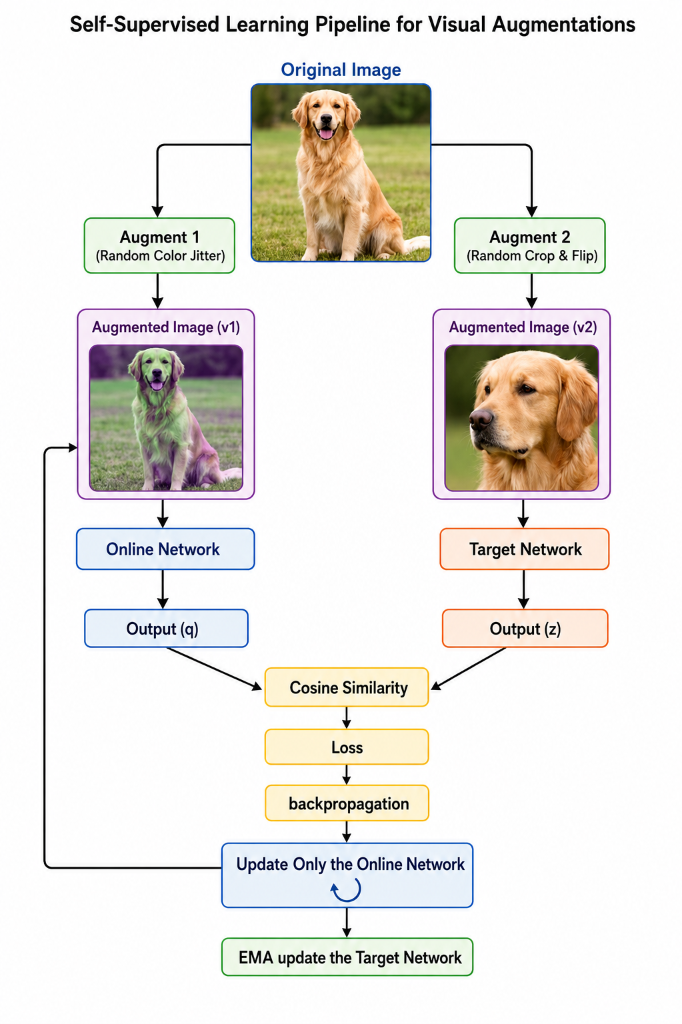
\includegraphics[width=0.82\textwidth]{figures/fig_7_byol_pipeline.png}
    \caption{Self-Supervised Learning Pipeline for Visual Augmentations in BYOL.}
    \label{fig:byol_pipeline}
\end{figure}

\subsection{Limitations of BYOL}

\begin{itemize}
    \item Requires two networks during training.
    \item Introduces EMA updates.
    \item Adds a Prediction Head, increasing architectural complexity.
    \item Initially lacked a complete theoretical explanation for why collapse does not occur.
\end{itemize}

\textbf{BYOL} successfully avoids representation collapse and achieves state-of-the-art performance, paving the way for later methods such as \textbf{SimSiam} and \textbf{DINO}.

\section{SimSiam (Simple Siamese Network)}

\textbf{BYOL} demonstrated that high-quality visual representations could be learned without negative samples. However, \textbf{BYOL} still required a Target Network updated via Exponential Moving Average (EMA), making the architecture more complex.

Researchers therefore asked an important question: \textbf{Is the momentum (EMA) Target Network really necessary?}

In 2021, Facebook AI introduced \textbf{SimSiam}, showing that self-supervised learning can still succeed without negative samples and without a momentum encoder. This was one of the most surprising discoveries in SSL.

By using a shared encoder, a Prediction Head, and a stop-gradient operation, it successfully learns meaningful visual representations without relying on negative samples or a memory queue. Its simplicity makes it one of the most elegant SSL methods and an important step toward later self-distillation approaches such as \textbf{DINO}.

\subsection{Main Idea of SimSiam}

The main idea of \textbf{SimSiam} is to learn by maximizing the similarity between augmented views of the same image.

Unlike \textbf{BYOL}:
\begin{itemize}
    \item No Momentum (EMA) Network
    \item No Memory Queue
    \item No Negative Samples
\end{itemize}

Instead, \textbf{SimSiam} relies on a shared Siamese network, a Prediction Head, and a Stop-Gradient operation to prevent collapse.

\subsection{Architecture}

\textbf{SimSiam} consists of two identical branches that share the same parameters.
Each branch contains:
\begin{itemize}
    \item Encoder
    \item Projection Head
\end{itemize}

For one direction of the loss, one branch passes through the Prediction Head and is compared with the stop-gradient output of the other branch. The full \textbf{SimSiam} algorithm then repeats this in the opposite direction.

\begin{figure}[H]
    \centering
    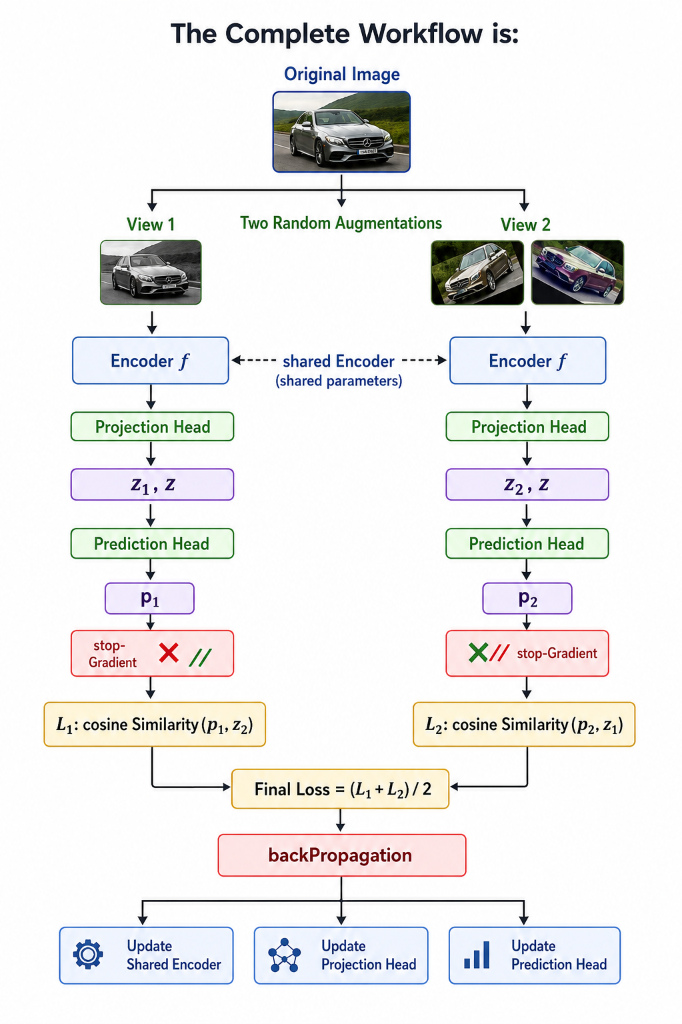
\includegraphics[width=0.82\textwidth]{figures/fig_7_simsiam_complete_workflow.png}
    \caption{The Complete Workflow of SimSiam.}
    \label{fig:simsiam_complete_workflow}
\end{figure}

\subsection{Splitting Architecture into 2 Branches}

Alternatively, we can split this architecture into two distinct loss branches:

\subsubsection{Loss $L_1$ Branch}
\begin{figure}[H]
    \centering
    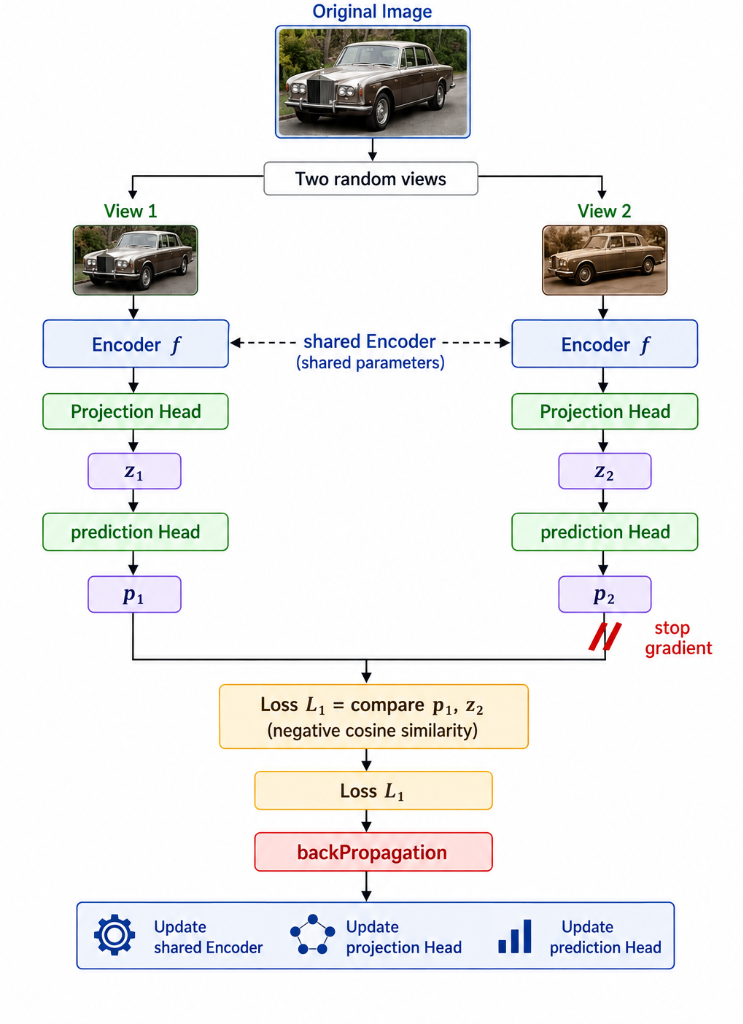
\includegraphics[width=0.78\textwidth]{figures/fig_7_simsiam_l1.png}
    \caption{SimSiam Loss $L_1$ Branch Architecture.}
    \label{fig:simsiam_l1}
\end{figure}

\subsubsection{Loss $L_2$ Branch}
\begin{figure}[H]
    \centering
    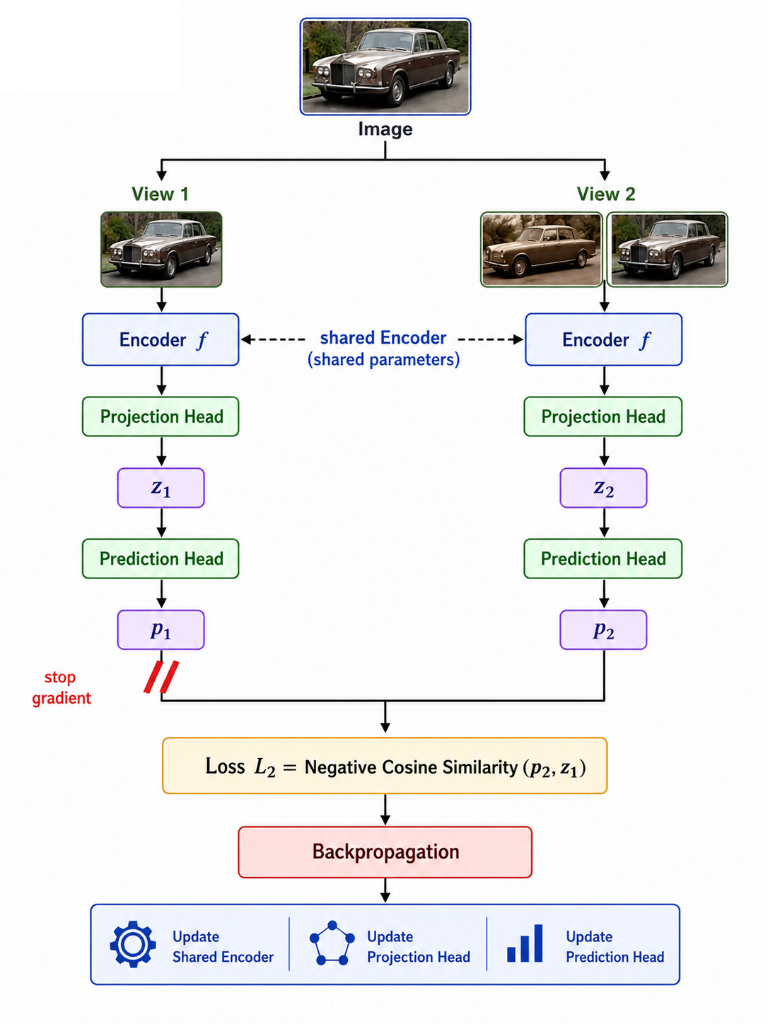
\includegraphics[width=0.78\textwidth]{figures/fig_7_simsiam_l2.png}
    \caption{SimSiam Loss $L_2$ Branch Architecture.}
    \label{fig:simsiam_l2}
\end{figure}

So \textbf{SimSiam} computes the loss symmetrically:
\begin{itemize}
    \item The first loss:
    \[
    L_1(p_1, z_2)
    \]
    \item Then the roles are swapped to compute the second loss:
    \[
    L_2(p_2, z_1)
    \]
\end{itemize}

Finally:
\[
L = \frac{L_1 + L_2}{2}
\]

\begin{itemize}
    \item $L_1$: compares prediction from branch 1 with the representation from branch 2 (after stop-gradient).
    \item $L_2$: compares prediction from branch 2 with the representation from branch 1 (after stop-gradient).
\end{itemize}

\subsection{Advantages of SimSiam}

\begin{itemize}
    \item Very Simple architecture.
    \item Only One encoder.
    \item No EMA update.
    \item No Memory Queue.
    \item No Negative Samples.
    \item Lower Computational Cost than \textbf{BYOL}.
    \item Competitive downstream performance.
\end{itemize}

\subsection{Limitations of SimSiam}

Despite its simplicity, \textbf{SimSiam} has some limitations:
\begin{itemize}
    \item More Sensitive to training settings than \textbf{BYOL}.
    \item Slightly lower performance than more recent methods such as \textbf{DINO}.
    \item Theoretical understanding of Collapse Prevention remains incomplete.
\end{itemize}

Although the precise theoretical explanation is still being studied, experiments show that removing the Stop Gradient causes the model to collapse.

\section{DINO (Distillation with No Labels)}

Although BYOL and SimSiam demonstrated that self-supervised learning could be performed without negative samples, researchers continued searching for methods capable of learning even richer visual representations.

In 2021, Facebook AI introduced \textbf{DINO} (\textbf{Di}stillation with \textbf{no} \textbf{L}abels). Instead of learning by directly matching representations, DINO adopts a teacher-student framework, where a student network learns to imitate a teacher network. Unlike traditional Knowledge Distillation, both networks are trained without labels, making the entire process self-supervised.

One of DINO's most remarkable discoveries is that the learned representations naturally capture object boundaries and semantic regions, allowing Vision Transformers to exhibit \textbf{emergent segmentation} without any segmentation labels.

Unlike BYOL, DINO predicts probability distributions rather than embeddings, and introduces Multi-Crop Training, Centering, and Sharpening to stabilize learning and avoid collapse. These innovations enable DINO to learn highly semantic visual representations and make it one of the most influential self-supervised learning methods for Vision Transformers.

\subsection{Main Idea of DINO}

The main idea of DINO is to train a student network to predict the output probability distribution produced by a teacher network for different augmented views of the same image.

Unlike BYOL:
\begin{itemize}
    \item The student predicts a probability distribution, not just an embedding.
    \item The teacher acts as a slowly evolving target.
    \item Additional mechanisms (Centering and Sharpening) stabilize training and prevent collapse.
\end{itemize}

DINO is therefore considered a \textbf{self-distillation} method.

\subsection{DINO Architecture}

DINO consists of two networks:
\begin{itemize}
    \item \textbf{Student Network}
    \item \textbf{Teacher Network}
\end{itemize}

Both networks contain:
\begin{enumerate}
    \item An Encoder (usually a Vision Transformer, ViT).
    \item A Projection Head.
\end{enumerate}

Unlike BYOL, neither network contains a separate prediction head. The teacher network is updated using an Exponential Moving Average (EMA) of the student network's parameters.
\clearpage
\begin{figure}[htbp]
    \centering
    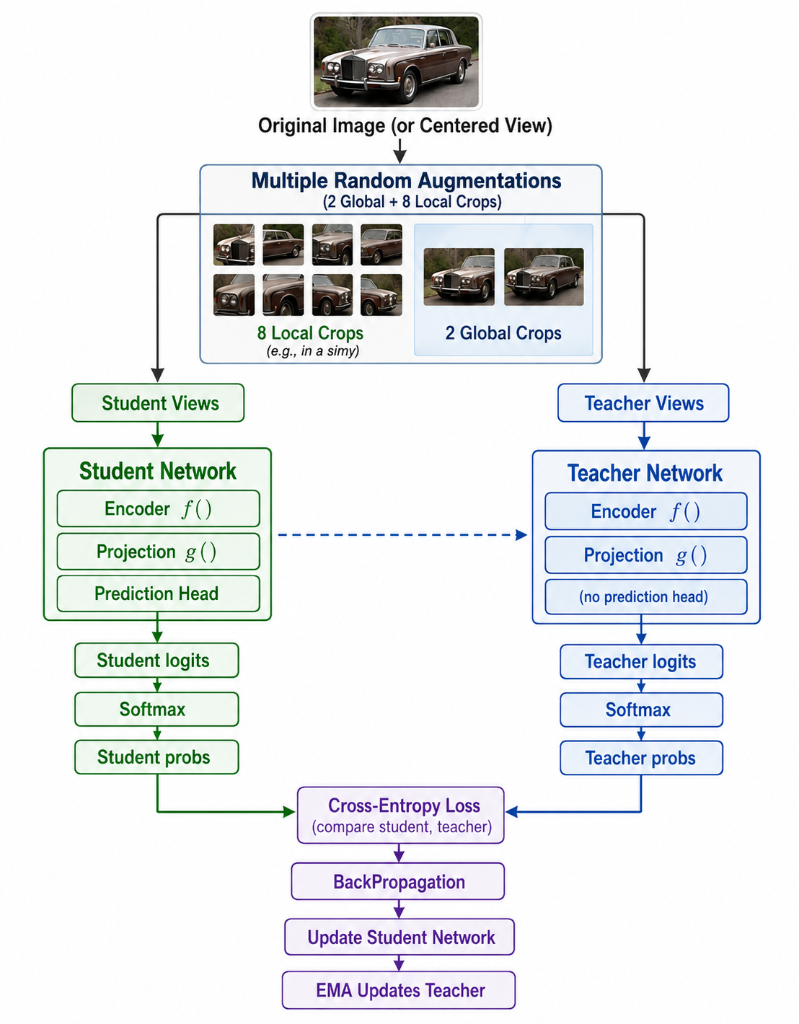
\includegraphics[width=0.85\linewidth]{figures/fig_7_dino_architecture.png}
    \caption{DINO Self-Distillation Architecture with Student and Teacher Networks.}
    \label{fig:dino_architecture}
\end{figure}

\subsection{Multi-Crop Training}

Before DINO, models learned that two global views correspond to the same object (e.g., entire cat $\rightarrow$ head, ear, or tail). A good representation should recognize that all these crops belong to the same object. Neither SimCLR nor BYOL explicitly enforced local-to-global view matching. This motivated DINO to introduce \textbf{Multi-Crop Training}.

Instead of generating only two views, DINO generates many views of an image:

\begin{figure}[htbp]
    \centering
    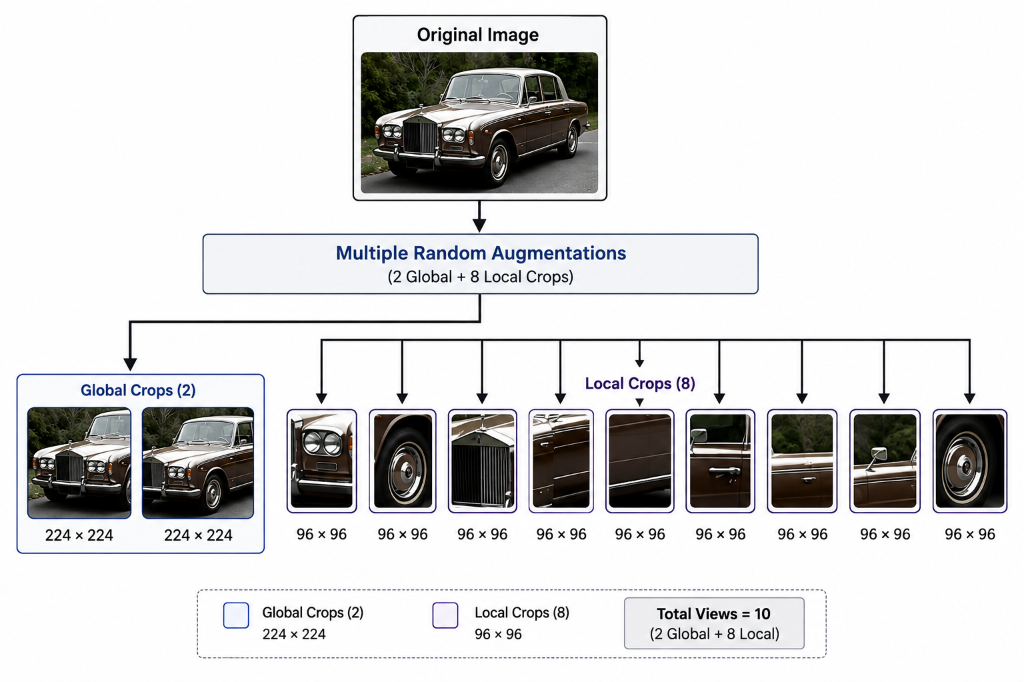
\includegraphics[width=0.9\linewidth]{figures/fig_7_dino_multicrop.png}
    \caption{DINO Multi-Crop Strategy with 2 Global Crops ($224 \times 224$) and 8 Local Crops ($96 \times 96$).}
    \label{fig:dino_multicrop}
\end{figure}

Typically, DINO creates:
\begin{itemize}
    \item \textbf{2 Global Crops}: Large crops ($224 \times 224$) covering most of the image, capturing global semantics.
    \item \textbf{8 Local Crops}: Small crops ($96 \times 96$) covering smaller regions (e.g., dog head, leg, or tail).
\end{itemize}

The student receives all crops (both global and local), while the teacher receives only global crops. The student must learn that local crops and global crops represent the same object, greatly improving representation robustness.

\subsection{Preventing Collapse: Centering and Sharpening}

While multi-crop training increases feature richness, another problem appears: the teacher network can start producing identical uniform outputs for every image, leading to representation collapse. To solve this, DINO introduces \textbf{Centering} and \textbf{Sharpening}.

\subsubsection{Centering}

Without centering, after many iterations, the teacher might output identical uniform distributions for all inputs (e.g., assigning 25\% probability to every class: Cat 25\%, Dog 25\%, Car 25\%, Bird 25\%). Every image receives the same prediction, causing the student to copy this trivial solution.

\textbf{The Solution (Centering):} DINO maintains a running average (center $c$) of the teacher's outputs across iterations. The center is subtracted from the teacher's logits before applying softmax:
\[
y_t = \text{Softmax}\left( \frac{g_t - c}{T_t} \right)
\]
where $g_t$ are the teacher logits, $c$ is the running center, and $T_t$ is the teacher temperature. Centering prevents any single dimension from dominating, encouraging the teacher to utilize the entire representation space.

\subsubsection{Sharpening}

While centering prevents collapse to a constant vector, it can cause the teacher's probability distribution to become overly soft (e.g., Cat 25\%, Dog 23\%, Car 22\%, Bird 20\%), leaving the student with an uninformative target.

\textbf{The Solution (Sharpening):} DINO applies a small temperature parameter $T_t < 1$ in the teacher's Softmax (e.g., $T_t = 0.04$ vs. $T=1.0$). Dividing by a small temperature scales up the largest logit, sharpening the distribution (e.g., turning probabilities like $[0.4, 0.26, 0.03, 0.01]$ into a decisive $[0.9999, 0.0001, 0, 0]$).

Combining Centering and Sharpening balances the predictions and keeps the teacher confident, producing a strong learning signal for the student.

\subsection{Loss Function}

The student predicts a probability distribution $P_s$, and the teacher produces a probability distribution $P_t$. The objective is to minimize the Cross-Entropy loss between them:
\[
\mathcal{L} = - \sum P_t \log P_s
\]
Unlike SimCLR or BYOL:
\begin{itemize}
    \item No Cosine Similarity.
    \item No InfoNCE loss.
    \item No Negative Samples.
\end{itemize}
The student simply learns to imitate the teacher's distribution.

\subsection{Emergent Segmentation}

One of DINO's most remarkable properties is that Vision Transformers (ViTs) trained with DINO naturally learn attention maps that align with object boundaries without any segmentation labels. The attention maps highlight:
\begin{itemize}
    \item Main objects.
    \item Semantic regions.
    \item Object contours.
\end{itemize}
This phenomenon is known as \textbf{emergent segmentation} and remains one of DINO's key milestones.

\subsection{Advantages and Limitations of DINO}

\textbf{Advantages:}
\begin{itemize}
    \item No labels required.
    \item No negative samples needed.
    \item Superior representations for Vision Transformers.
    \item Multi-scale learning via multi-crop training.
    \item Emergent segmentation capabilities.
    \item Strong performance on downstream transfer tasks.
\end{itemize}

\textbf{Limitations:}
\begin{itemize}
    \item More complex than BYOL and SimSiam.
    \item Requires delicate hyperparameter tuning for Centering and Sharpening.
    \item Higher computational cost due to multi-crop training (10 views per image).
\end{itemize}

\section{DINOv2}

The original DINO demonstrated that self-distillation could learn excellent visual representations without labels. However, it was trained on relatively small datasets compared to modern foundation models.

In 2023, Meta introduced \textbf{DINOv2} to answer a fundamental question: \emph{Can DINO become a general-purpose vision foundation model, similar to how GPT became a foundation model for language?}

Rather than proposing a completely new learning algorithm, DINOv2 focuses on scaling up the DINO framework using carefully curated data, larger ViT architectures, and optimized training techniques.

\subsection{Automatic Dataset Curation}

A core innovation of DINOv2 is its automatic data curation pipeline. Instead of uncurated web scraping, Meta built an automated pipeline to clean and balance a massive image repository by removing:
\begin{itemize}
    \item Duplicate images.
    \item Low-quality or corrupted images.
    \item Watermarked images.
    \item Near-identical copies and noisy samples.
\end{itemize}
This resulted in a clean, diverse dataset (LVD-142M), proving that data quality is as important as model architecture.

\subsection{Large-Scale Training and Downstream Tasks}

DINOv2 was trained on hundreds of millions of curated images. The resulting representations transfer seamlessly across diverse computer vision tasks without task-specific fine-tuning:
\begin{itemize}
    \item Image Classification \& Retrieval
    \item Object Detection \& Instance Segmentation
    \item Depth Estimation \& Semantic Segmentation
    \item Few-shot and Zero-shot Learning
\end{itemize}

\section{Masked Image Modeling (MIM)}

Until now, all self-supervised methods studied (SimCLR, MoCo, BYOL, SimSiam, DINO) belong to the view-comparison family: learning by contrasting or matching two augmented views of an image.

Researchers proposed a fundamentally different approach: \emph{Can a model learn visual representations by reconstructing missing parts of an image instead of comparing two full images?} This idea gave birth to \textbf{Masked Image Modeling (MIM)}.

\begin{figure}[htbp]
    \centering
    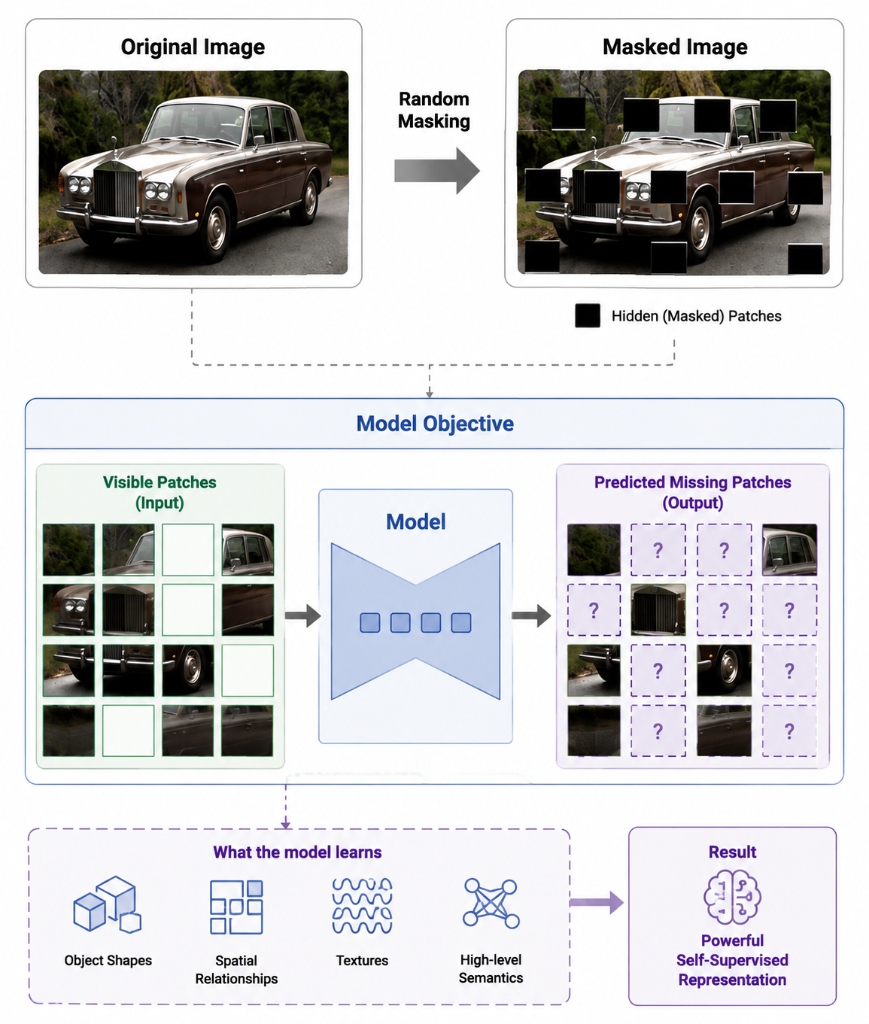
\includegraphics[width=0.85\linewidth]{figures/fig_7_mim_objective.jpg}
    \caption{Masked Image Modeling (MIM) Objective: predicting hidden patches from visible context.}
    \label{fig:mim_objective}
\end{figure}

\subsection{Main Idea of MIM}

Instead of feeding a complete image, MIM intentionally hides (masks) a large percentage of image patches (e.g., 40\%--75\%). The model receives only the visible patches and must infer the missing regions.

To predict the hidden patches accurately, the model must understand:
\begin{itemize}
    \item Object shapes and boundaries.
    \item Spatial relationships.
    \item Textures and high-level semantics.
\end{itemize}

Since the original unmasked image already contains the ground-truth content, supervision comes directly from the image itself—making MIM a pure self-supervised task.

\subsection{Target Prediction Types in MIM}

Different MIM architectures target different representation formats:
\begin{itemize}
    \item \textbf{BEiT}: Predicts discrete \textbf{visual tokens}.
    \item \textbf{MAE}: Reconstructs raw \textbf{pixel values}.
    \item \textbf{iBOT}: Combines patch reconstruction with self-distillation.
\end{itemize}

\section{BEiT (BERT Pre-Training of Image Transformers)}

Introduced by Microsoft, \textbf{BEiT} adapts BERT's masked language modeling concept to computer vision. Often referred to as \emph{"BERT for Images"}, BEiT masks image patches and trains a Vision Transformer to predict discrete visual tokens generated by a pretrained, frozen visual tokenizer (dVAE).

\subsection{From BERT to BEiT}

In NLP, BERT masks words in a sentence and predicts them:
\[
\text{The cat is [MASK] on the sofa} \longrightarrow \text{predict: sleeping}
\]
BEiT operates identically for images: it masks a subset of image patches and predicts the corresponding visual token for each masked patch.

\subsection{Visual Tokens}

A visual token is analogous to a word ID in NLP vocabulary. For example, in BERT, $\text{cat} \rightarrow \text{Token ID 384}$. In BEiT, an image patch (e.g., a dog's ear) is mapped by a Discrete VAE (dVAE) tokenizer into a discrete token ID (e.g., $\text{Token 812}$).

Instead of predicting millions of raw RGB values, BEiT predicts discrete token IDs that represent high-level visual concepts.

\subsection{BEiT Architecture}

BEiT consists of two separate components:
\begin{enumerate}
    \item \textbf{Visual Tokenizer (Frozen)}: Pretrained dVAE that converts image patches into discrete visual tokens. Its weights are fixed during BEiT training.
    \item \textbf{Vision Transformer (Trainable)}: Processes masked patch embeddings and predicts the missing visual token IDs.
\end{enumerate}
\clearpage
\begin{figure}[htbp]
    \centering
    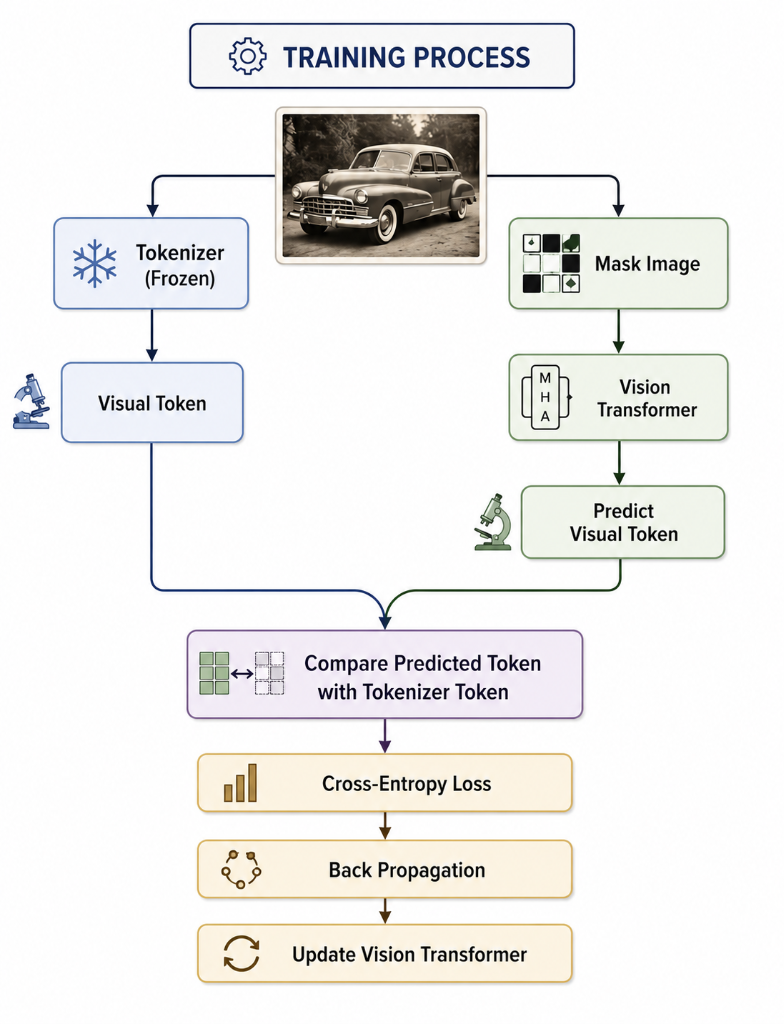
\includegraphics[width=0.85\linewidth]{figures/fig_7_beit_training_process.png}
    \caption{BEiT Training Process with Frozen Tokenizer and Trainable Vision Transformer.}
    \label{fig:beit_training_process}
\end{figure}

\subsection{Loss Function}

Since the target is a discrete token ID, BEiT uses standard \textbf{Cross-Entropy Loss} between the predicted token probability distribution and the ground-truth token ID produced by the frozen tokenizer.

\subsection{Why Predict Tokens Instead of Pixels?}

Predicting raw pixel values is highly ambiguous: a masked sky patch could have many valid RGB color shades. In contrast, predicting a visual token forces the model to focus on abstract semantic categories rather than low-level pixel noise.

\subsection{Advantages and Limitations of BEiT}

\textbf{Advantages:}
\begin{itemize}
    \item Learns high-level semantic representations.
    \item Directly leverages BERT's proven masked modeling paradigm.
    \item Avoids pixel reconstruction ambiguity.
    \item Delivers strong transfer performance on vision tasks.
\end{itemize}

\textbf{Limitations:}
\begin{itemize}
    \item Requires a separate pretrained visual tokenizer (dVAE).
    \item Two-stage training pipeline (stage 1: train tokenizer; stage 2: train BEiT).
    \item Performance is bounded by tokenizer quality.
    \item Additional computational complexity from the tokenizer.
\end{itemize}

\subsection{MAE (Masked Autoencoders)}

Although BEiT achieved excellent performance, it introduced a new fundamental question: \emph{why do we need a separate visual tokenizer?} Training the tokenizer requires an additional model, extra computation, and a two-stage training pipeline.

Researchers at Meta (He et al., 2021) asked a simpler question: \textbf{Can we remove the tokenizer completely and directly reconstruct missing image patches?}

The answer was \textbf{MAE (Masked Autoencoders)}. MAE demonstrated that simply reconstructing missing raw pixels is sufficient to learn powerful visual representations—provided the architecture is designed asymmetrically and efficiently.

\subsubsection{Key Simplification}

MAE simplifies Masked Image Modeling by eliminating the pretrained visual tokenizer. Instead, it:
\begin{enumerate}
    \item Masks a very high proportion of image patches (approximately \textbf{75\%}).
    \item Trains a Vision Transformer encoder on only the remaining \textbf{25\% visible patches}.
    \item Uses a lightweight decoder to reconstruct the original pixel values of the missing patches.
    \item Minimizes reconstruction error using \textbf{Mean Squared Error (MSE)}.
\end{enumerate}

Unlike BEiT, MAE uses:
\begin{itemize}
    \item No visual tokenizer.
    \item No visual token vocabulary.
    \item Direct pixel-level reconstruction.
\end{itemize}

\subsubsection{Why a 75\% Masking Ratio?}

One of MAE's most surprising insights is its extremely high masking ratio. While NLP models like BERT mask 15\% of words and early vision methods masked $\sim$40\%, MAE masks \textbf{75\% of all image patches}, leaving only 25\% visible.


This high masking ratio is necessary because images contain immense spatial redundancy. For example, in an image of a dog, even if most of the image is covered, a human can easily infer the missing parts from surrounding context. A low masking ratio (e.g., 15\%) makes the reconstruction task trivial, allowing the model to extrapolate pixels locally without learning deep semantic structure. Masking 75\% forces the model to understand global scene composition.

\subsubsection{Asymmetric Encoder-Decoder Architecture}

MAE introduces a novel asymmetric design where the heavy encoder only sees visible patches:

\begin{itemize}
    \item \textbf{Encoder}: A standard Vision Transformer that processes \emph{only} unmasked visible patches (25\%). Masked patches are completely discarded before the encoder. This reduces computational cost dramatically (roughly a $4\times$ reduction in FLOPs).
    \item \textbf{Decoder}: A lightweight Transformer that receives the latent representations of visible patches plus shared learnable \textbf{Mask Tokens} (`[MASK]`) for missing positions. It reconstructs full-resolution RGB pixels. The decoder is discarded after pretraining.
\end{itemize}
\clearpage
\begin{figure}[htbp]
    \centering
    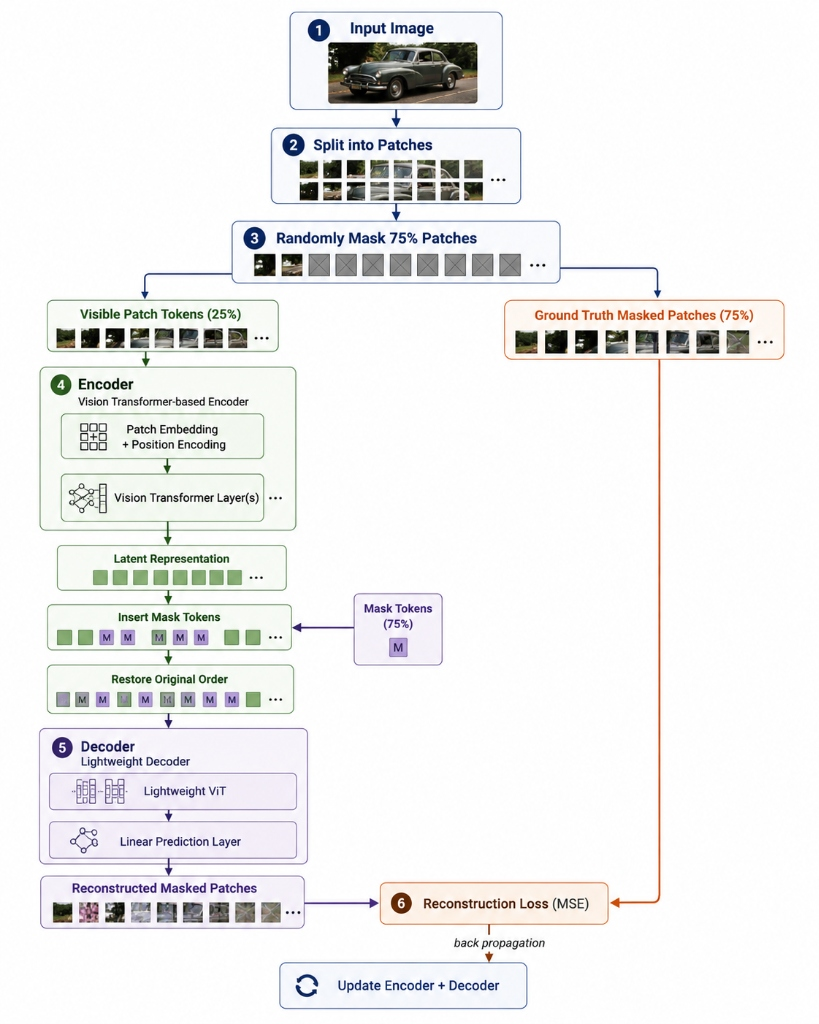
\includegraphics[width=0.85\linewidth]{figures/fig_7_mae_architecture.png}
    \caption{MAE Architecture: Processing only 25\% visible patches through the encoder, inserting mask tokens, and reconstructing raw pixels with a lightweight decoder.}
    \label{fig:mae_architecture}
\end{figure}

\subsubsection{Reconstruction Loss}

The reconstruction loss is the Mean Squared Error (MSE) between predicted pixel values $\hat{x}_i$ and original RGB pixels $x_i$, computed exclusively over masked patches $M$:
\[
\mathcal{L}_{\text{MSE}} = \frac{1}{|M|} \sum_{i \in M} \|x_i - \hat{x}_i\|^2
\]

\subsubsection{Fine-Tuning}

After pretraining, the lightweight decoder is removed. The pretrained ViT encoder is retained and fine-tuned for downstream computer vision tasks such as:
\begin{itemize}
    \item Image Classification.
    \item Object Detection.
    \item Semantic Segmentation.
\end{itemize}

\subsubsection{Advantages of MAE}
\begin{itemize}
    \item \textbf{No Visual Tokenizer}: Eliminates dVAE pretraining and complex tokenizers.
    \item \textbf{High Efficiency}: Asymmetric design allows processing only $25\%$ of patches in the encoder.
    \item \textbf{Strong Semantics}: High masking ratio forces global conceptual reasoning.
    \item \textbf{Scalability}: Scales exceptionally well to massive ViT models (ViT-Huge, ViT-Giant).
\end{itemize}

\subsection{iBOT (Image BERT with Online Tokenizer)}

By late 2021, self-supervised learning for vision had divided into two distinct paradigms:
\begin{enumerate}
    \item \textbf{Distillation-based Methods} (BYOL, SimSiam, DINO): Excel at learning \textbf{global image representations} by enforcing consistency between augmented views.
    \item \textbf{Masked Image Modeling} (BEiT, MAE): Excel at learning \textbf{local patch representations} by reconstructing missing regions.
\end{enumerate}

Researchers at ByteDance (Zhou et al., 2021) asked: \emph{Can we combine the strengths of both paradigms?} This led to \textbf{iBOT (Image BERT with Online Tokenizer)}, which unifies self-distillation and masked image modeling in a single framework.

\begin{figure}[htbp]
    \centering
    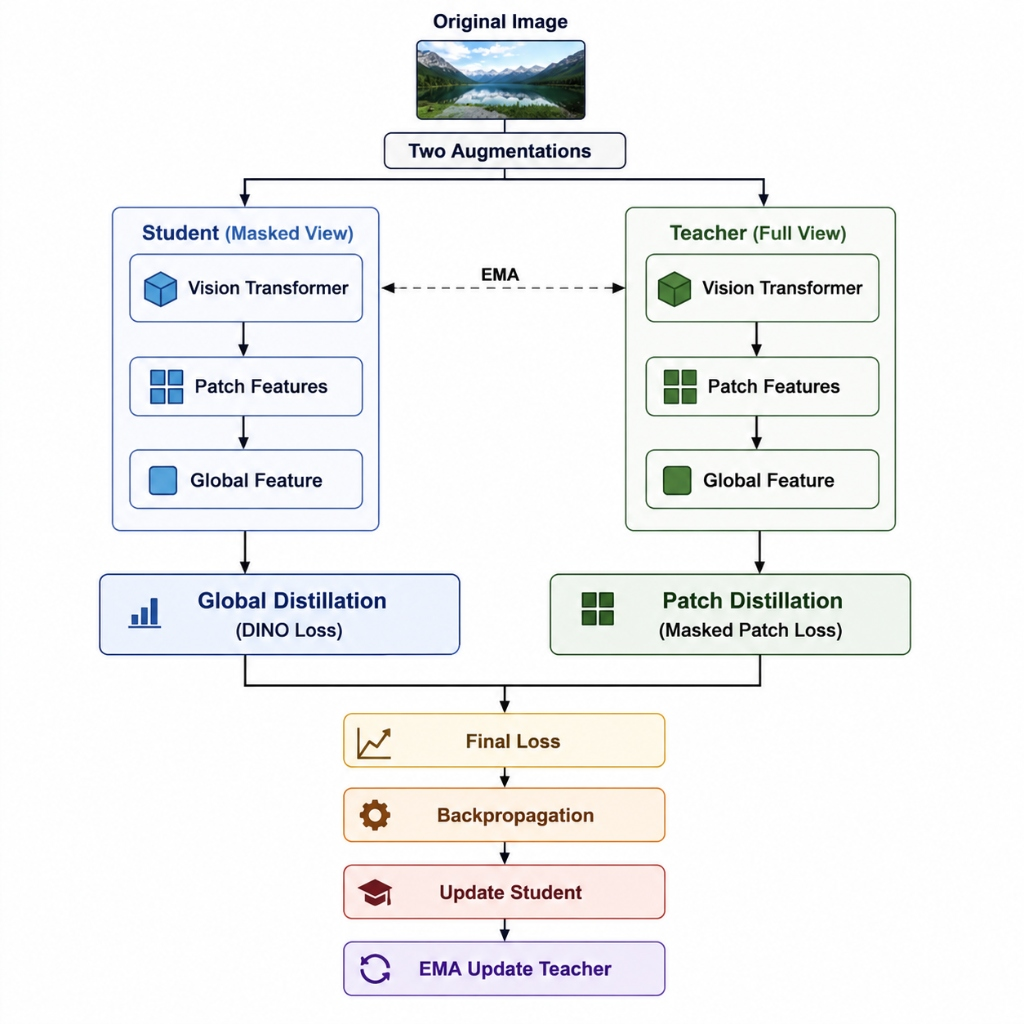
\includegraphics[width=0.85\linewidth]{figures/fig_7_ibot_overview.png}
    \caption{iBOT High-Level Overview: Combining Global Distillation (DINO Loss) and Patch Distillation (Masked Patch Loss).}
    \label{fig:ibot_overview}
\end{figure}

\subsubsection{Main Idea}

Instead of choosing between global consistency and local reconstruction, iBOT performs both simultaneously:
\begin{itemize}
    \item \textbf{Global Task}: Learns a global representation for the entire image (like DINO).
    \item \textbf{Patch Task}: Learns detailed semantic representations for individual masked patches (like BEiT/MAE).
\end{itemize}

For example, when given an image of a dog:
\begin{itemize}
    \item DINO learns: \emph{"This entire scene is a dog"} (Global).
    \item MAE learns: \emph{"This hidden patch should be RGB $(125, 117, 110)$"} (Local pixel).
    \item \textbf{iBOT learns both}: \emph{"This image is a dog"} AND \emph{"This hidden patch represents a dog's ear"} (Semantic patch representation).
\end{itemize}

\begin{figure}[htbp]
    \centering
    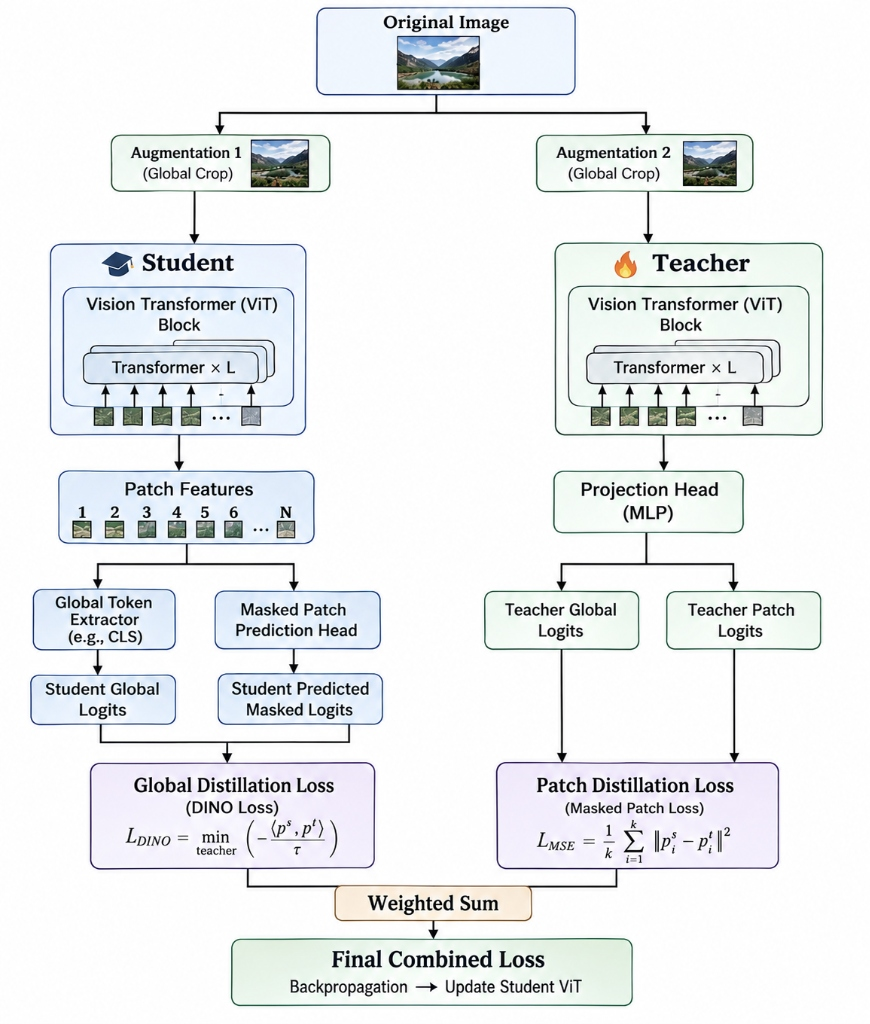
\includegraphics[width=0.9\linewidth]{figures/fig_7_ibot_detailed.jpg}
    \caption{Detailed iBOT Teacher-Student Learning Framework.}
    \label{fig:ibot_detailed}
\end{figure}

\subsubsection{iBOT Architecture \& Targets}

iBOT employs a DINO-like Student-Teacher setup:
\begin{itemize}
    \item \textbf{Teacher Network}: Processes the unmasked full image and generates semantic targets for both the global image and individual patches. Updated via Exponential Moving Average (EMA).
    \item \textbf{Student Network}: Processes masked views of the image and learns to predict both global logits and teacher patch features simultaneously.
\end{itemize}

Crucially, \textbf{iBOT does not reconstruct raw pixels (unlike MAE) nor predict discrete token IDs (unlike BEiT)}. Instead, the student predicts the \textbf{teacher's high-level patch feature representations}.

\subsubsection{iBOT Loss Function}

iBOT optimizes a dual objective:
\[
\mathcal{L}_{\text{iBOT}} = \mathcal{L}_{\text{global}} + \mathcal{L}_{\text{patch}}
\]
\begin{itemize}
    \item $\mathcal{L}_{\text{global}}$: Cross-entropy loss matching student global representation to teacher global representation (DINO loss).
    \item $\mathcal{L}_{\text{patch}}$: Cross-entropy loss matching student masked patch predictions to corresponding teacher patch representations.
\end{itemize}

\subsubsection{Advantages and Limitations}
\textbf{Advantages:}
\begin{itemize}
    \item Unifies global image semantics and fine-grained local patch understanding.
    \item Self-conditioned online tokenizer eliminates the need for an offline dVAE.
    \item Outperforms previous SSL methods on dense prediction tasks (segmentation, detection).
\end{itemize}

\textbf{Limitations:}
\begin{itemize}
    \item Higher computational complexity (requires Teacher, Student, EMA, and dual losses).
    \item More memory-intensive training pipeline.
\end{itemize}


\section{Modern Self-Supervised Learning Frontiers}

Self-supervised learning continues to evolve rapidly. This section highlights four cutting-edge frameworks that shaped modern representation learning.

\subsection{Barlow Twins (Learning by Reducing Redundancy)}

Proposed by Zbontar et al. (2021), \textbf{Barlow Twins} addresses a central question: \emph{Can we learn effective representations without negative pairs, teacher networks, queues, or pixel reconstruction?}

\begin{figure}[htbp]
    \centering
    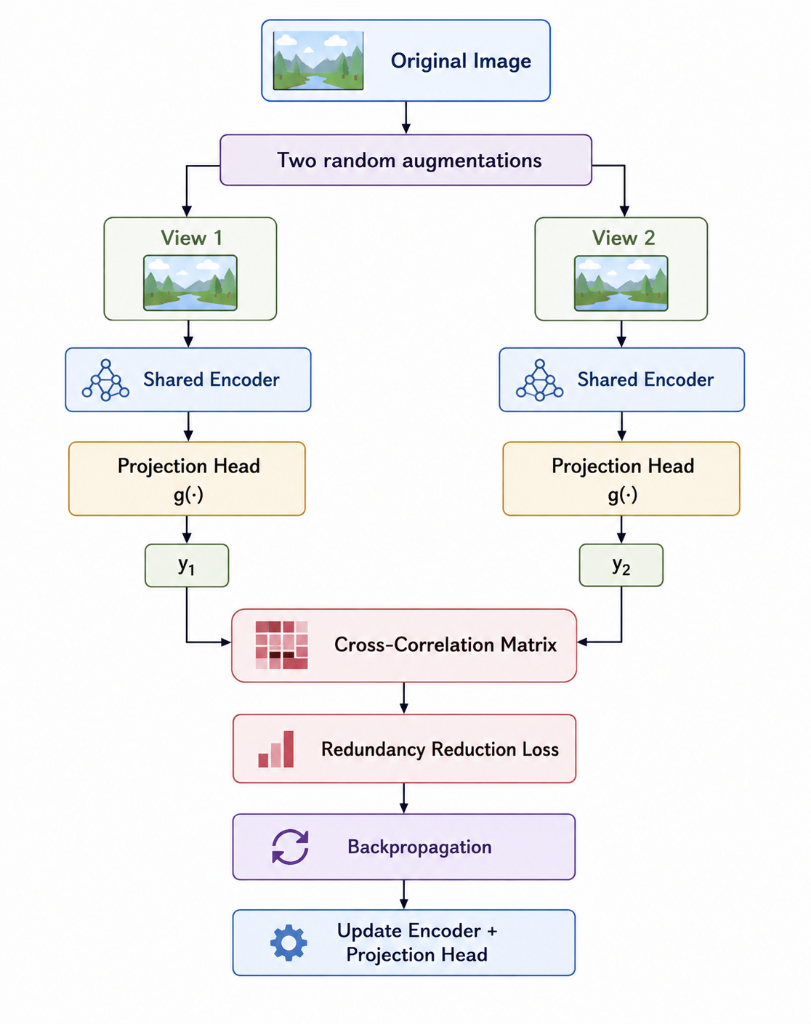
\includegraphics[width=0.85\linewidth]{figures/fig_7_barlow_twins.png}
    \caption{Barlow Twins Architecture: Computing the Cross-Correlation Matrix between twin representations to enforce Redundancy Reduction.}
    \label{fig:barlow_twins}
\end{figure}

Barlow Twins applies neuroscience-inspired \textbf{redundancy reduction} to representation learning.

\subsubsection{Core Principle}

Given two augmented views $y_1, y_2$ of the same image processed through a shared encoder and projection head, Barlow Twins computes their normalized \textbf{Cross-Correlation Matrix} $\mathcal{C}$:
\[
\mathcal{C}_{ij} = \frac{\sum_b z_{b,i}^{(1)} z_{b,j}^{(2)}}{\sqrt{\sum_b (z_{b,i}^{(1)})^2} \sqrt{\sum_b (z_{b,j}^{(2)})^2}}
\]
where $b$ indexes batch samples, and $i, j$ index vector feature dimensions.

The objective forces $\mathcal{C}$ to resemble the Identity matrix $I$:
\begin{itemize}
    \item \textbf{Diagonal Elements ($\mathcal{C}_{ii} \to 1$)}: \emph{Invariance term}—forces the same feature component to be invariant to data augmentations.
    \item \textbf{Off-Diagonal Elements ($\mathcal{C}_{ij} \to 0, i \neq j$)}: \emph{Redundancy Reduction term}—decorrelates different feature components, ensuring each vector entry captures unique, independent information.
\end{itemize}

The loss function is defined as:
\[
\mathcal{L}_{\text{BT}} = \sum_i (1 - \mathcal{C}_{ii})^2 + \lambda \sum_i \sum_{j \neq i} \mathcal{C}_{ij}^2
\]
\vspace{5cm}

\subsection{VICReg (Variance, InVariance, Covariance)}

Proposed by Bardes et al. (2021), \textbf{VICReg} expands on non-contrastive learning by explicitly decomposing representation regularization into three explicit terms.
\clearpage
\begin{figure}[htbp]
    \centering
    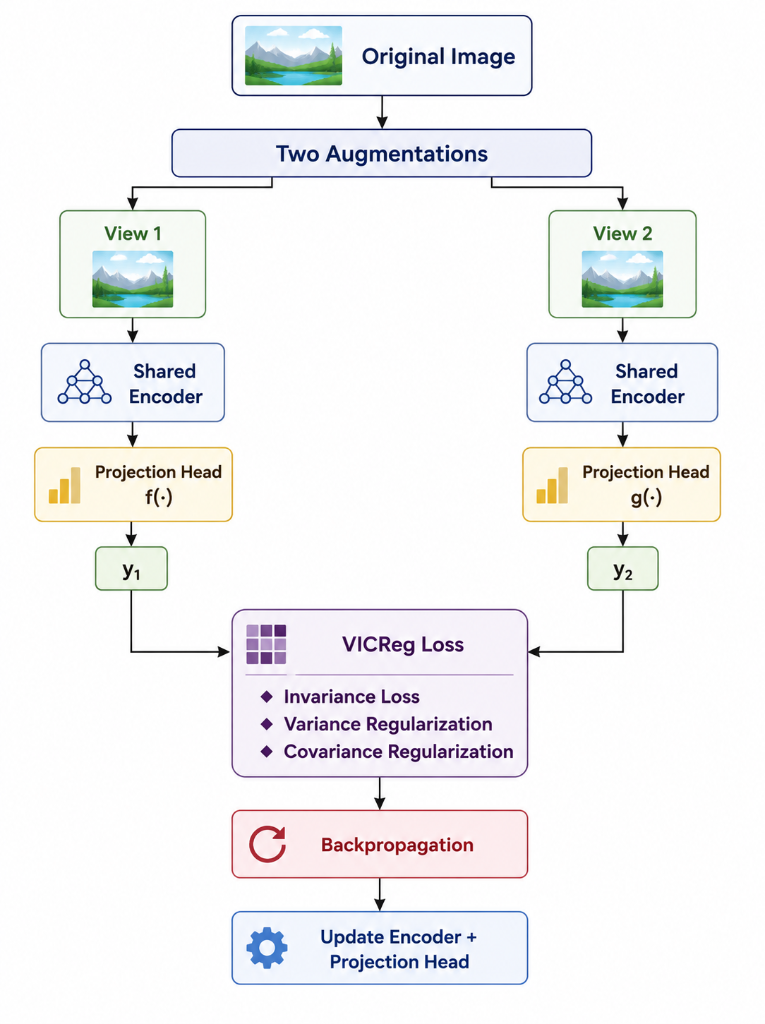
\includegraphics[width=0.85\linewidth]{figures/fig_7_vicreg_architecture.png}
    \caption{VICReg Architecture: Explicitly optimizing Invariance Loss, Variance Regularization, and Covariance Regularization.}
    \label{fig:vicreg}
\end{figure}

\clearpage
\vspace{5cm}
VICReg avoids representation collapse without negative pairs or asymmetric teacher architectures by enforcing three criteria directly on representations $Z_1, Z_2$:
\begin{enumerate}
    \item \textbf{Invariance ($s$)}: Standard mean squared error between representations of augmented views.
    \item \textbf{Variance ($v$)}: Hinge loss forcing the standard deviation of each feature dimension across a batch to remain above a threshold $\gamma > 0$ (prevents feature collapse to a constant).
    \item \textbf{Covariance ($c$)}: Off-diagonal covariance matrix penalty, decorrelating different features to eliminate redundancy.
\end{enumerate}

\[
\mathcal{L}_{\text{VICReg}} = \lambda s(Z_1, Z_2) + \mu [v(Z_1) + v(Z_2)] + \nu [c(Z_1) + c(Z_2)]
\]

VICReg is widely valued for its mathematical simplicity, stability, and absence of asymmetric architectural tricks.
\vspace{5cm}

\subsection{I-JEPA (Image Joint-Embedding Predictive Architecture)}

Proposed by Yann LeCun and Meta AI (Assran et al., 2023), \textbf{I-JEPA} (Image Joint-Embedding Predictive Architecture) addresses a fundamental limitation of pixel-reconstruction models such as MAE: \emph{Predicting every pixel forces the model to allocate capacity to unpredictable, low-level details (e.g., exact textures or noise), which are often irrelevant for learning high-level semantic representations.}

\clearpage
\begin{figure}[htbp]
    \centering
    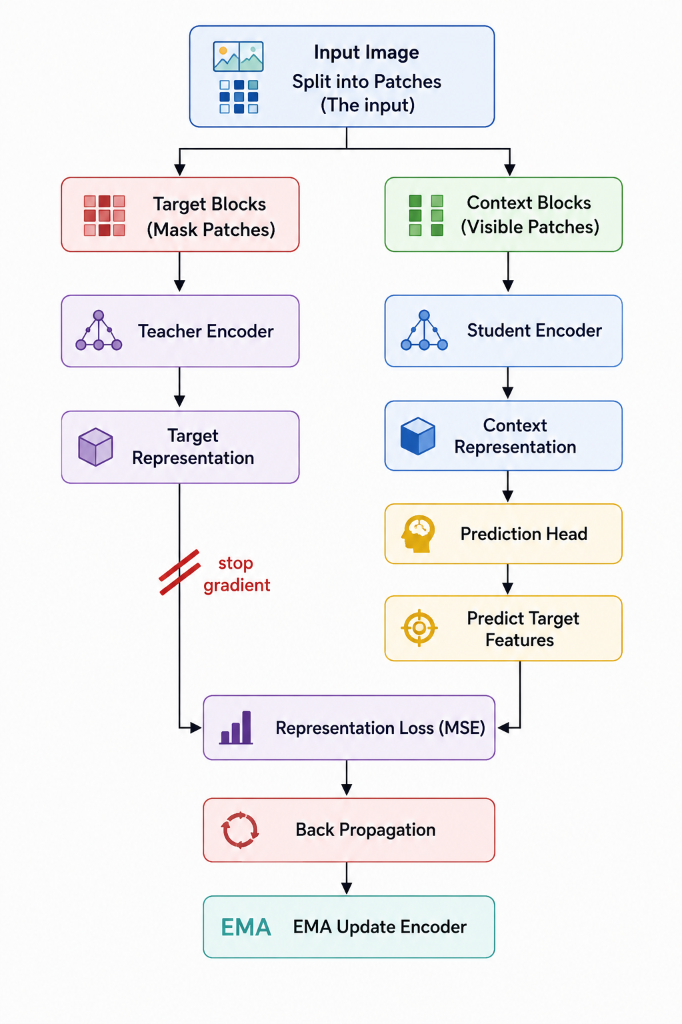
\includegraphics[width=0.85\linewidth]{figures/fig_7_ijepa_architecture.png}
    \caption{I-JEPA architecture: predicting target representations from visible context representations in the embedding space.}
    \label{fig:ijepa}
\end{figure}
\clearpage

\subsubsection{Main Idea}

Instead of reconstructing pixels in the image space, \textbf{I-JEPA predicts high-level semantic representations directly in the embedding space}.

\begin{itemize}
    \item \textbf{Context Blocks} (visible image patches) are processed by a \textbf{Student Encoder} to produce context embeddings.
    
    \item \textbf{Target Blocks} (masked image regions) are processed by a \textbf{Teacher Encoder} (with stop-gradient) to produce target embeddings.
    
    \item A \textbf{Predictor} receives the context embeddings together with the positional embeddings of the target blocks and predicts the corresponding target embeddings.
    
    \item \textbf{Training Objective:} Minimize the Mean Squared Error (MSE) between the predicted target embeddings and the target embeddings produced by the Teacher Encoder.
\end{itemize}

By predicting semantic representations rather than reconstructing pixels, \textbf{I-JEPA} learns meaningful high-level features while avoiding unnecessary focus on unpredictable low-level image details. This enables the model to learn more robust and semantically rich visual representations for downstream tasks.


\vspace{5cm}
\subsection{CLIP (Contrastive Language-Image Pre-training)}

Introduced by OpenAI (Radford et al., 2021), \textbf{CLIP} bridges computer vision and natural language processing using multimodal contrastive learning.
\clearpage
\begin{figure}[htbp]
    \centering
    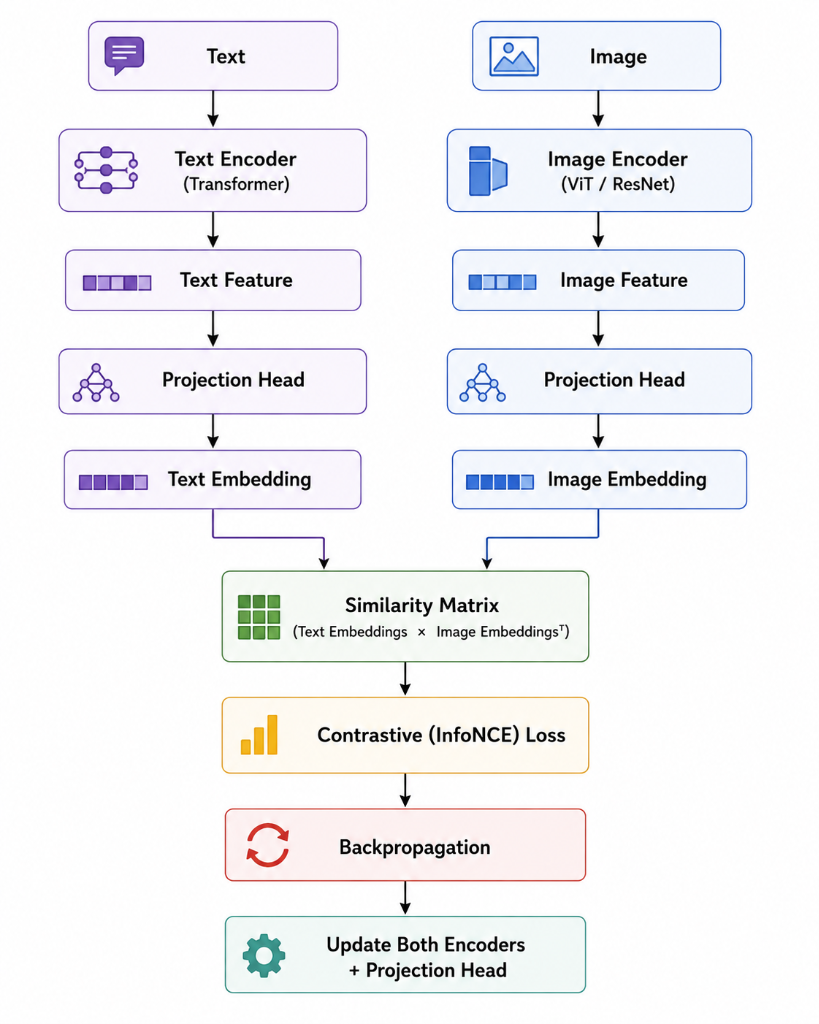
\includegraphics[width=0.85\linewidth]{figures/fig_7_clip_architecture.png}
    \caption{CLIP Multimodal Contrastive Learning Architecture.}
    \label{fig:clip}
\end{figure}
\clearpage

\vspace{5cm}
\subsubsection{Main Idea}

CLIP jointly trains an \textbf{Image Encoder} (ViT or ResNet) and a \textbf{Text Encoder} (Transformer) on 400 million (image, text) pairs curated from the internet.

Given a batch of $N$ (image, text) pairs:
\begin{enumerate}
    \item Images are encoded into image embeddings $I_1, I_2, \dots, I_N$.
    \item Text prompts are encoded into text embeddings $T_1, T_2, \dots, T_N$.
    \item An $N \times N$ similarity matrix is computed via cosine similarity: $S_{i,j} = \text{sim}(I_i, T_j)$.
    \item Symmetric InfoNCE loss maximizes similarity along the diagonal ($I_i, T_i$) while minimizing off-diagonal pairs ($I_i, T_j, i \neq j$).
\end{enumerate}

\subsubsection{Zero-Shot Classification}

The key breakthrough of CLIP is \textbf{Zero-Shot Transfer}. After pretraining, CLIP can perform image classification without any task-specific fine-tuning:
\begin{enumerate}
    \item Text prompts are created for each target class (e.g., \emph{"a photo of a [dog]"}, \emph{"a photo of a [cat]"}).
    \item Prompt text embeddings are generated using the Text Encoder.
    \item The test image embedding is matched against all text prompt embeddings via cosine similarity.
    \item The class corresponding to the highest similarity score is selected as the prediction.
\end{enumerate}

CLIP's robust zero-shot capabilities established it as the foundation for modern multimodal systems, including Stable Diffusion, DALL-E 2, and vision-LLMs.
